\chapter{\protect\hyperlink{:}{热学}}
\addtocontents{toc}{\protect\hypertarget{:}{}}


热学从两个角度研究热现象：\textbf{宏观}角度（热力学）和\textbf{微观}角度（统计物理）。热力学通过实验总结出基本定律，不涉及微观机制；统计物理则从大量粒子的集体行为出发，用概率和统计的方法推导出宏观规律。两条路径殊途同归，互为补充。


\section{\protect\hyperlink{:}{气体状态参量与温标}}
\addtocontents{toc}{\protect\hypertarget{:}{}}

\subsection{\protect\hyperlink{:}{气体的状态参量}}
\addtocontents{toc}{\protect\hypertarget{:}{}}

要描述一个热力学系统的宏观状态，我们需要一组\textbf{状态参量}。对于一定量的气体，最基本的状态参量有三个：

\begin{enumerate}
    \item \textbf{压强 $p$}：气体对容器壁单位面积上的压力，国际单位为帕斯卡（Pa），$1\text{ Pa} = 1\text{ N/m}^2$。
    \item \textbf{体积 $V$}：气体所占据的空间，国际单位为立方米（m$^3$）。
    \item \textbf{温度 $T$}：表征物体冷热程度的物理量，其严格定义需要依赖热力学第零定律。
\end{enumerate}

当一个系统处于平衡态时，其状态参量不随时间变化，且处处均匀。此时三个参量之间存在一个确定的关系——\textbf{状态方程}。对于理想气体，状态方程为
\begin{equation}
    pV = \nu RT
\end{equation}

其中 $\nu$ 为物质的量（摩尔数），$R = 8.314$ J/(mol$\cdot$K) 为理想气体常量。

\subsection{\protect\hyperlink{:}{热力学第零定律与温标}}
\addtocontents{toc}{\protect\hypertarget{:}{}}

在定义温度之前，我们先需要明确"两个系统温度相等"意味着什么。

\begin{theorem}[热力学第零定律]
    如果系统 $A$ 和系统 $B$ 分别与系统 $C$ 处于热平衡，则 $A$ 和 $B$ 之间也处于热平衡。
\end{theorem}

第零定律告诉我们，存在一个可以用来判断热平衡的状态量——这就是\textbf{温度}。当两个系统温度相等时，它们之间没有净热量传递。

为了定量地测量温度，我们需要建立\textbf{温标}——即温度的数值标度。

\subsubsection{\protect\hyperlink{:}{理想气体温标}}
\addtocontents{toc}{\protect\hypertarget{:}{}}

理想气体温标基于理想气体的性质建立。由理想气体状态方程 $pV = \nu RT$，当体积不变时
\begin{equation}
    p \propto T
\end{equation}

利用这一关系，我们可以定义温度的比值。选取水的三相点（固态、液态、气态三相共存）为参考点，规定其温度为 $T_3 = 273.16$ K，则任意温度 $T$ 定义为
\begin{equation}
    T = 273.16 \text{ K} \times \frac{p}{p_3}
\end{equation}

其中 $p$ 是一定量气体在体积不变时的压强，$p_3$ 是该气体在三相点时的压强。

\subsubsection{\protect\hyperlink{:}{摄氏温标与华氏温标}}
\addtocontents{toc}{\protect\hypertarget{:}{}}

日常中常用的摄氏温标 $t$ 与热力学温度 $T$ 的关系为
\begin{equation}
    t(\text{°C}) = T(\text{K}) - 273.15
\end{equation}

华氏温标 $t_F$ 与摄氏温标的关系为
\begin{equation}
    t_F(\text{°F}) = \frac{9}{5}t(\text{°C}) + 32
\end{equation}

\subsubsection{\protect\hyperlink{:}{热力学温标}}
\addtocontents{toc}{\protect\hypertarget{:}{}}

热力学温标是建立在热力学第二定律基础上的温标，它不依赖于任何具体物质的性质。可以证明，在理想气体温标适用的范围内，热力学温标与理想气体温标完全一致。热力学温标的零点（$T = 0$ K）称为\textbf{绝对零度}，是理论上能达到的最低温度。


\section{\protect\hyperlink{:}{热力学第一定律}}
\addtocontents{toc}{\protect\hypertarget{:}{}}

\subsection{\protect\hyperlink{:}{功与热量}}
\addtocontents{toc}{\protect\hypertarget{:}{}}

热力学系统与外界交换能量的方式有两种：\textbf{做功}和\textbf{传热}。

\subsubsection{\protect\hyperlink{:}{功}}
\addtocontents{toc}{\protect\hypertarget{:}{}}

当气体的体积发生变化时，气体对外界做功（或外界对气体做功）。考虑一个装有气体的气缸，活塞面积为 $S$，气体压强为 $p$，当活塞移动 $\mathrm{d}x$ 时，气体对外做的功为
\begin{equation}
    \mathrm{d}W = F\,\mathrm{d}x = pS\,\mathrm{d}x = p\,\mathrm{d}V
\end{equation}

气体从状态 $A$（体积 $V_A$）变化到状态 $B$（体积 $V_B$）时，气体对外做的总功为
\begin{equation}
    W = \int_{V_A}^{V_B} p\,\mathrm{d}V
\end{equation}

在 $p$-$V$ 图上，功等于过程曲线下方的面积。

\begin{remark}
    功是\textbf{过程量}，不是状态量。从同一个初态到同一个末态，不同的过程做功一般不同。
\end{remark}

\subsubsection{\protect\hyperlink{:}{热量}}
\addtocontents{toc}{\protect\hypertarget{:}{}}

当系统与外界存在温度差时，能量会以\textbf{热传递}的方式从高温物体流向低温物体。传递的能量称为\textbf{热量}，记作 $Q$。

\begin{remark}
    热量也是\textbf{过程量}，不是状态量。"一个物体含有多少热量"这种说法是错误的。
\end{remark}

\subsection{\protect\hyperlink{:}{热力学第一定律}}
\addtocontents{toc}{\protect\hypertarget{:}{}}

热力学第一定律本质上是能量守恒定律在热力学中的表述。

\begin{theorem}[热力学第一定律]
    一个系统从外界吸收的热量 $Q$，一部分用于增加系统的内能 $\Delta U$，另一部分用于对外做功 $W$
    \begin{equation}
        Q = \Delta U + W
    \end{equation}
    其中各量的符号约定：$Q > 0$ 表示系统吸热，$Q < 0$ 表示系统放热；$W > 0$ 表示系统对外做功，$W < 0$ 表示外界对系统做功；$\Delta U > 0$ 表示内能增加。
\end{theorem}

对于一个无穷小的过程
\begin{equation}
    \mathrm{d}Q = \mathrm{d}U + \mathrm{d}W = \mathrm{d}U + p\,\mathrm{d}V
\end{equation}

\begin{remark}
    内能 $U$ 是\textbf{状态量}，只与系统的状态有关，与过程无关。对于理想气体，内能只是温度的函数 $U = U(T)$。
\end{remark}

\subsection{\protect\hyperlink{:}{热容}}
\addtocontents{toc}{\protect\hypertarget{:}{}}

\begin{definition}[热容]
    系统在某一过程中温度升高 1 K 所吸收的热量称为该过程的热容
    \begin{equation}
        C = \frac{\mathrm{d}Q}{\mathrm{d}T}
    \end{equation}
\end{definition}

常用的有两个热容：
\begin{enumerate}
    \item \textbf{定容热容} $C_V$：体积不变时的热容。由于 $\mathrm{d}W = p\,\mathrm{d}V = 0$，所以 $\mathrm{d}Q = \mathrm{d}U$，即
    \begin{equation}
        C_V = \left(\frac{\partial U}{\partial T}\right)_V
    \end{equation}
    \item \textbf{定压热容} $C_p$：压强不变时的热容。由热力学第一定律
    \begin{equation}
        C_p = \left(\frac{\partial U}{\partial T}\right)_V + p\left(\frac{\partial V}{\partial T}\right)_p
    \end{equation}
\end{enumerate}

对于理想气体，$C_p$ 与 $C_V$ 之间有如下关系（迈耶公式）
\begin{equation}
    C_p - C_V = \nu R
\end{equation}

\subsection{\protect\hyperlink{:}{理想气体的典型过程}}
\addtocontents{toc}{\protect\hypertarget{:}{}}

\subsubsection{\protect\hyperlink{:}{等体过程}}
\addtocontents{toc}{\protect\hypertarget{:}{}}

体积不变（$V = \text{常量}$），$\mathrm{d}W = 0$，所以 $Q = \Delta U$。在 $p$-$V$ 图上是一条竖直线。

由查理定律
\begin{equation}
    \frac{p}{T} = \text{常量}
\end{equation}

\subsubsection{\protect\hyperlink{:}{等压过程}}
\addtocontents{toc}{\protect\hypertarget{:}{}}

压强不变（$p = \text{常量}$），在 $p$-$V$ 图上是一条水平线。

由盖-吕萨克定律
\begin{equation}
    \frac{V}{T} = \text{常量}
\end{equation}

气体对外做功 $W = p\Delta V = \nu R\Delta T$。

\subsubsection{\protect\hyperlink{:}{等温过程}}
\addtocontents{toc}{\protect\hypertarget{:}{}}

温度不变（$T = \text{常量}$），对于理想气体，$\Delta U = 0$，所以 $Q = W$。

由玻意耳定律
\begin{equation}
    pV = \text{常量}
\end{equation}

在 $p$-$V$ 图上是一条双曲线（等温线）。气体对外做功为
\begin{equation}
    W = \nu RT\ln\frac{V_2}{V_1}
\end{equation}

\subsubsection{\protect\hyperlink{:}{绝热过程}}
\addtocontents{toc}{\protect\hypertarget{:}{}}

系统与外界没有热量交换（$Q = 0$），所以 $\Delta U = -W$。气体对外做功以消耗内能为代价，温度下降。

可以证明，理想气体的绝热过程满足
\begin{equation}
    pV^\gamma = \text{常量}
\end{equation}

其中 $\gamma = C_p/C_V$ 为比热容比。在 $p$-$V$ 图上，绝热线比等温线更陡。


\section{\protect\hyperlink{:}{卡诺循环与热机效率}}
\addtocontents{toc}{\protect\hypertarget{:}{}}

\subsection{\protect\hyperlink{:}{循环过程}}
\addtocontents{toc}{\protect\hypertarget{:}{}}

\textbf{热机}的工作原理是：从高温热源吸收热量，对外做功，同时向低温热源放出热量。工作物质经历一个\textbf{循环过程}后回到初态。

\begin{definition}[热机效率]
    热机的效率定义为对外做的净功与从高温热源吸收的热量之比
    \begin{equation}
        \eta = \frac{W}{Q_1} = \frac{Q_1 - Q_2}{Q_1} = 1 - \frac{Q_2}{Q_1}
    \end{equation}
    其中 $Q_1$ 是从高温热源吸收的热量，$Q_2$ 是向低温热源放出的热量（取绝对值）。
\end{definition}

\subsection{\protect\hyperlink{:}{卡诺循环}}
\addtocontents{toc}{\protect\hypertarget{:}{}}

卡诺循环是由法国工程师卡诺在 1824 年提出的理想热机循环，它由两个等温过程和两个绝热过程组成。

\begin{figure}[htbp]
    \centering
    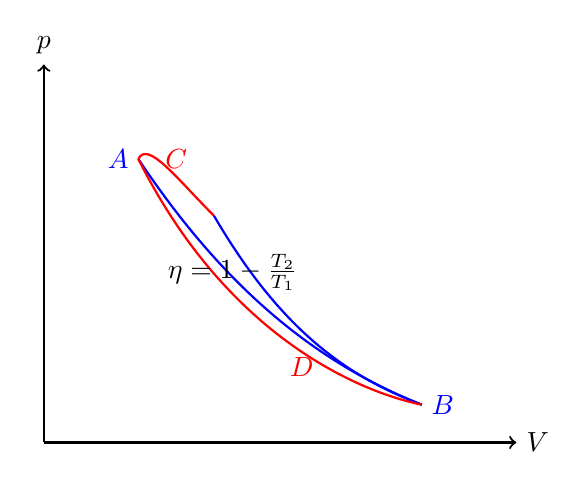
\begin{tikzpicture}[scale=1.2]
        \draw[->,thick] (0,0) -- (5,0) node[right]{$V$};
        \draw[->,thick] (0,0) -- (0,4) node[above]{$p$};
        \draw[thick,blue] (1,3) .. controls (2,1.5) and (3,0.8) .. (4,0.4);
        \node[left,blue] at (1,3) {$A$};
        \draw[thick,blue] (4,0.4) .. controls (3.2,0.7) and (2.5,1.2) .. (1.8,2.4);
        \node[right,blue] at (4,0.4) {$B$};
        \draw[thick,red] (1.8,2.4) .. controls (1.4,2.8) and (1.1,3.2) .. (1,3);
        \node[above,red] at (1.4,2.8) {$C$};
        \draw[thick,red] (4,0.4) .. controls (3.5,0.5) and (2,1) .. (1,3);
        \node[below right,red] at (2.5,1) {$D$};
        \node at (2,1.8) {$\eta = 1 - \frac{T_2}{T_1}$};
    \end{tikzpicture}
    \caption{卡诺循环示意图}
    \label{fig:卡诺循环}
\end{figure}

卡诺循环的四个过程：
\begin{enumerate}
    \item \textbf{等温膨胀}（$A \to B$，温度 $T_1$）：气体从高温热源 $T_1$ 吸收热量 $Q_1$，等温膨胀对外做功。
    \item \textbf{绝热膨胀}（$B \to C$）：气体绝热膨胀，温度从 $T_1$ 降到 $T_2$，对外做功。
    \item \textbf{等温压缩}（$C \to D$，温度 $T_2$）：气体被等温压缩，向低温热源 $T_2$ 放出热量 $Q_2$。
    \item \textbf{绝热压缩}（$D \to A$）：气体被绝热压缩，温度从 $T_2$ 升回 $T_1$。
\end{enumerate}

可以计算出卡诺热机的效率为
\begin{equation}
    \eta_{\text{卡诺}} = 1 - \frac{T_2}{T_1}
\end{equation}

其中 $T_1$、$T_2$ 分别是高温热源和低温热源的热力学温度。

\begin{remark}
    卡诺定理：在相同的高温热源和低温热源之间工作的一切热机，可逆热机的效率最高，且所有可逆热机的效率相同，与工作物质无关。这表明 $1 - T_2/T_1$ 是热机效率的上限。
\end{remark}

\subsection{\protect\hyperlink{:}{制冷机}}
\addtocontents{toc}{\protect\hypertarget{:}{}}

如果让卡诺循环反向运行，就变成了\textbf{制冷机}：外界对系统做功 $W$，从低温热源吸收热量 $Q_2$，向高温热源放出热量 $Q_1 = Q_2 + W$。

\begin{definition}[制冷系数]
    制冷机的制冷系数定义为
    \begin{equation}
        \varepsilon = \frac{Q_2}{W} = \frac{Q_2}{Q_1 - Q_2}
    \end{equation}
\end{definition}

卡诺制冷机的制冷系数为
\begin{equation}
    \varepsilon_{\text{卡诺}} = \frac{T_2}{T_1 - T_2}
\end{equation}


\section{\protect\hyperlink{:}{热力学第二定律}}
\addtocontents{toc}{\protect\hypertarget{:}{}}

\subsection{\protect\hyperlink{:}{两种表述}}
\addtocontents{toc}{\protect\hypertarget{:}{}}

热力学第一定律告诉我们能量守恒，但它没有告诉我们过程的\textbf{方向性}。例如，热量自发地从高温物体传到低温物体，但不会自发地反向传递——这种方向性由热力学第二定律来描述。

\begin{theorem}[热力学第二定律]
    \begin{enumerate}
        \item \textbf{开尔文表述}：不可能从单一热源吸收热量，使之完全变为功，而不引起其他变化。（即：第二类永动机不可能实现。）
        \item \textbf{克劳修斯表述}：热量不可能自发地从低温物体传到高温物体，而不引起其他变化。
    \end{enumerate}
\end{theorem}

两种表述是等价的。如果违反开尔文表述，就可以构造出违反克劳修斯表述的系统，反之亦然。

\begin{remark}
    热力学第二定律的实质是：自然界中一切与热现象有关的宏观过程都是\textbf{不可逆的}。这种不可逆性源于大量粒子的统计行为。
\end{remark}


\section{\protect\hyperlink{:}{熵}}
\addtocontents{toc}{\protect\hypertarget{:}{}}

\subsection{\protect\hyperlink{:}{熵的引入}}
\addtocontents{toc}{\protect\hypertarget{:}{}}

热力学第二定律表明，不可逆过程有方向性。为了定量地描述这种方向性，我们引入一个新的状态函数——\textbf{熵}。

考虑一个可逆过程，系统从状态 $A$ 变化到状态 $B$。可以证明，积分 $\int_A^B \frac{\mathrm{d}Q_{\text{可逆}}}{T}$ 的值与路径无关，只与初末状态有关。因此我们可以定义一个状态函数：

\begin{definition}[熵]
    系统从状态 $A$ 到状态 $B$ 的熵变为
    \begin{equation}
        \Delta S = S_B - S_A = \int_A^B \frac{\mathrm{d}Q_{\text{可逆}}}{T}
    \end{equation}
    对于无穷小的可逆过程
    \begin{equation}
        \mathrm{d}S = \frac{\mathrm{d}Q_{\text{可逆}}}{T}
    \end{equation}
\end{definition}

\subsection{\protect\hyperlink{:}{熵增加原理}}
\addtocontents{toc}{\protect\hypertarget{:}{}}

对于不可逆过程，可以证明
\begin{equation}
    \mathrm{d}S > \frac{\mathrm{d}Q_{\text{不可逆}}}{T}
\end{equation}

将可逆和不可逆过程合并，得到\textbf{克劳修斯不等式}
\begin{equation}
    \oint \frac{\mathrm{d}Q}{T} \leqslant 0
\end{equation}

等号对应可逆过程，不等号对应不可逆过程。

由此得到\textbf{熵增加原理}：

\begin{theorem}[熵增加原理]
    在绝热过程（或孤立系统）中，系统的熵永不减少
    \begin{equation}
        \Delta S \geqslant 0
    \end{equation}
    等号对应可逆过程，不等号对应不可逆过程。
\end{theorem}

熵增加原理给出了宏观过程进行方向的判据：在孤立系统中，过程总是朝着熵增加的方向进行，直到熵达到最大值——此时系统达到平衡态。

\subsection{\protect\hyperlink{:}{熵的统计意义}}
\addtocontents{toc}{\protect\hypertarget{:}{}}

玻尔兹曼给出了熵的统计解释：

\begin{equation}
    S = k_B \ln\Omega
\end{equation}

其中 $k_B = 1.381 \times 10^{-23}$ J/K 为玻尔兹曼常量，$\Omega$ 是系统在给定宏观状态下的\textbf{微观状态数}。

这个公式揭示了熵的微观本质：熵是系统\textbf{无序程度}的度量。微观状态数越多，系统的无序程度越高，熵越大。


\section{\protect\hyperlink{:}{相变}}
\addtocontents{toc}{\protect\hypertarget{:}{}}

\subsection{\protect\hyperlink{:}{相与相变}}
\addtocontents{toc}{\protect\hypertarget{:}{}}

\begin{definition}[相]
    物质在热力学平衡态下存在的不同聚集态称为\textbf{相}。例如，水的固相（冰）、液相（水）、气相（水蒸气）。
\end{definition}

当外界条件（温度、压强）变化时，物质可以从一个相转变为另一个相——这就是\textbf{相变}。

\subsection{\protect\hyperlink{:}{克拉珀龙方程}}
\addtocontents{toc}{\protect\hypertarget{:}{}}

在 $p$-$T$ 相图上，两相共存的平衡条件由\textbf{克拉珀龙方程}描述：

\begin{theorem}[克拉珀龙方程]
    在两相平衡曲线上，压强随温度的变化率为
    \begin{equation}
        \frac{\mathrm{d}p}{\mathrm{d}T} = \frac{L}{T\Delta V}
    \end{equation}
    其中 $L$ 为相变潜热（单位质量的物质在相变过程中吸收或放出的热量），$\Delta V$ 为相变前后单位质量的体积变化。
\end{theorem}

\subsection{\protect\hyperlink{:}{一级相变与二级相变}}
\addtocontents{toc}{\protect\hypertarget{:}{}}

\subsubsection{\protect\hyperlink{:}{一级相变}}
\addtocontents{toc}{\protect\hypertarget{:}{}}

\textbf{一级相变}的特征是：相变时有潜热的吸收或放出，且体积发生突变。克拉珀龙方程描述的就是一级相变。

常见的一级相变有：冰的融化、水的汽化、升华等。

对于汽液相变，利用克拉珀龙方程可以推导出\textbf{克拉修斯-克拉珀龙方程}
\begin{equation}
    \frac{\mathrm{d}p}{\mathrm{d}T} = \frac{L}{T(V_g - V_l)} \approx \frac{Lp}{RT^2}
\end{equation}

其中近似条件为：气相可看作理想气体，且 $V_g \gg V_l$。积分后得到
\begin{equation}
    \ln p = -\frac{L}{RT} + C
\end{equation}

这表明 $\ln p$ 与 $1/T$ 近似成线性关系。

\subsubsection{\protect\hyperlink{:}{二级相变}}
\addtocontents{toc}{\protect\hypertarget{:}{}}

\textbf{二级相变}的特征是：没有潜热，没有体积突变，但热容、压缩率等物理量发生突变。

常见的二级相变有：铁磁-顺磁转变（居里点）、超导转变等。

\subsection{\protect\hyperlink{:}{相律}}
\addtocontents{toc}{\protect\hypertarget{:}{}}

\begin{theorem}[吉布斯相律]
    对于一个有 $C$ 个独立组分、$\Phi$ 个相共存的系统，其自由度为
    \begin{equation}
        f = C - \Phi + 2
    \end{equation}
    其中 $f$ 是可以独立变化的强度变量的数目。
\end{theorem}

例如，对于纯水（$C = 1$）：
\begin{enumerate}
    \item 单相区（$\Phi = 1$）：$f = 2$，温度和压强可以独立变化。
    \item 两相共存（$\Phi = 2$）：$f = 1$，温度和压强中只有一个可以独立变化（即沿相变曲线）。
    \item 三相点（$\Phi = 3$）：$f = 0$，温度和压强都确定。
\end{enumerate}
